%; whizzy chapter
% -initex iniptex -latex platex -format platex -bibtex jbibtex -fmt fmt
% 以上 whizzytex を使用する場合の設定。

%     Kansai Debian Meeting resources
%     Copyright (C) 2007 Takaya Yamashita
%     Thank you for Tokyo Debian Meeting resources

%     This program is free software; you can redistribute it and/or modify
%     it under the terms of the GNU General Public License as published by
%     the Free Software Foundation; either version 2 of the License, or
%     (at your option) any later version.

%     This program is distributed in the hope that it will be useful,
%     but WITHOUT ANY WARRANTY; without even the implied warranty of
%     MERCHANTABILITY or FITNESS FOR A PARTICULAR PURPOSE.  See the
%     GNU General Public License for more details.

%     You should have received a copy of the GNU General Public License
%     along with this program; if not, write to the Free Software
%     Foundation, Inc., 51 Franklin St, Fifth Floor, Boston, MA  02110-1301 USA

%  preview (shell-command (concat "evince " (replace-regexp-in-string "tex$" "pdf"(buffer-file-name)) "&"))
% 画像ファイルを処理するためにはebbを利用してboundingboxを作成。
%(shell-command "cd image200708; ebb *.png")

%%ここからヘッダ開始。

\documentclass[mingoth,a4paper]{jsarticle}
\usepackage{kansaimonthlyreport}
\usepackage[dvips]{xy}
\usepackage{ascmac}

% 日付を定義する、毎月変わります。
\newcommand{\debmtgyear}{2010}
\newcommand{\debmtgdate}{26}
\newcommand{\debmtgmonth}{12}
\newcommand{\debmtgnumber}{42}

\begin{document}

\begin{titlepage}

% 毎月変更する部分、本文の末尾も修正することをわすれずに

 第\debmtgnumber{}回 関西 Debian 勉強会資料

\vspace{2cm}

\begin{center}
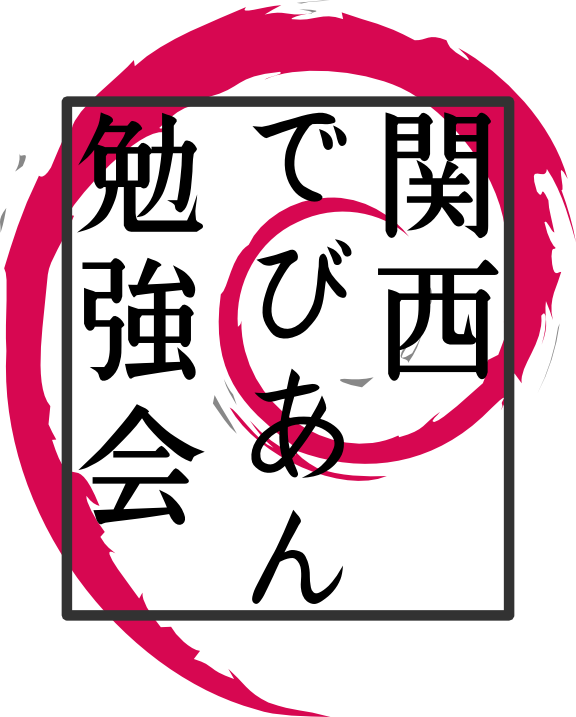
\includegraphics{image200802/kansaidebianlogo.png}
\end{center}

\begin{flushright}
\hfill{}関西 Debian 勉強会担当者 佐々木・倉敷・のがた \\
\hfill{}\debmtgyear{}年\debmtgmonth{}月\debmtgdate{}日
\end{flushright}

\thispagestyle{empty}
\end{titlepage}

\dancersection{Introduction}{Debian JP}

\subsection*{}%ロゴ用のスペース稼ぎ

関西 Debian 勉強会はDebian GNU/Linux のさまざまなトピック(新しいパッケー
ジ、Debian 特有の機能の仕組、Debian 界隈で起こった出来事、などなど)に
ついて話し合う会です。

目的として次の三つを考えています。
\begin{itemize}
      \item MLや掲示板ではなく、直接顔を合わせる事での情報交換の促進
      \item 定期的に集まれる場所
      \item 資料の作成
\end{itemize}

それでは、楽しい一時をお楽しみ下さい。

\clearpage

\begin{minipage}[b]{0.2\hsize}
 {\rotatebox{90}{\fontsize{80}{80}
{\gt 関西 Debian 勉強会}}}
\end{minipage}
\begin{minipage}[b]{0.8\hsize}
\hrule
\vspace{2mm}
\hrule
\setcounter{tocdepth}{1}
\tableofcontents
\vspace{2mm}
\hrule
\end{minipage}

\dancersection{最近のDebian関係のイベント報告}{Debian JP}

\subsection{第 41 回関西 Debian 勉強会@関西オープンソース2010}

前回の関西 Debian 勉強会は、11月5日、6日に開催された関西オープンソース
2010にてブース出展とセッションをおこないました。

ブースでは、準備不足もあってDebian LiveをネットワークブートしDebianを体験
してもらうコーナーについては見せられませんでしたが、東京からやまねさん、
吉田さんが参加されたり、UbuntuやGentoo、Emacs勉強会の方々も訪れたりして交
流を深めました。

セッションでは、第41回関西Debian勉強会「でびあん らんだむ とぴっくす」と
して佐々木さんによるSqueezeリリース状況や最近のDebian関連の動きなどについ
ての発表と、急遽お願いして発表していただいた矢吹さんのベトナムで行われた
Mini DebConfの報告がありました。

Squeezeはリリースが近いこともりあり、参加された方々も興味深く聞き入ってた
ようでした。

\begin{figure}[h]
    \centering
    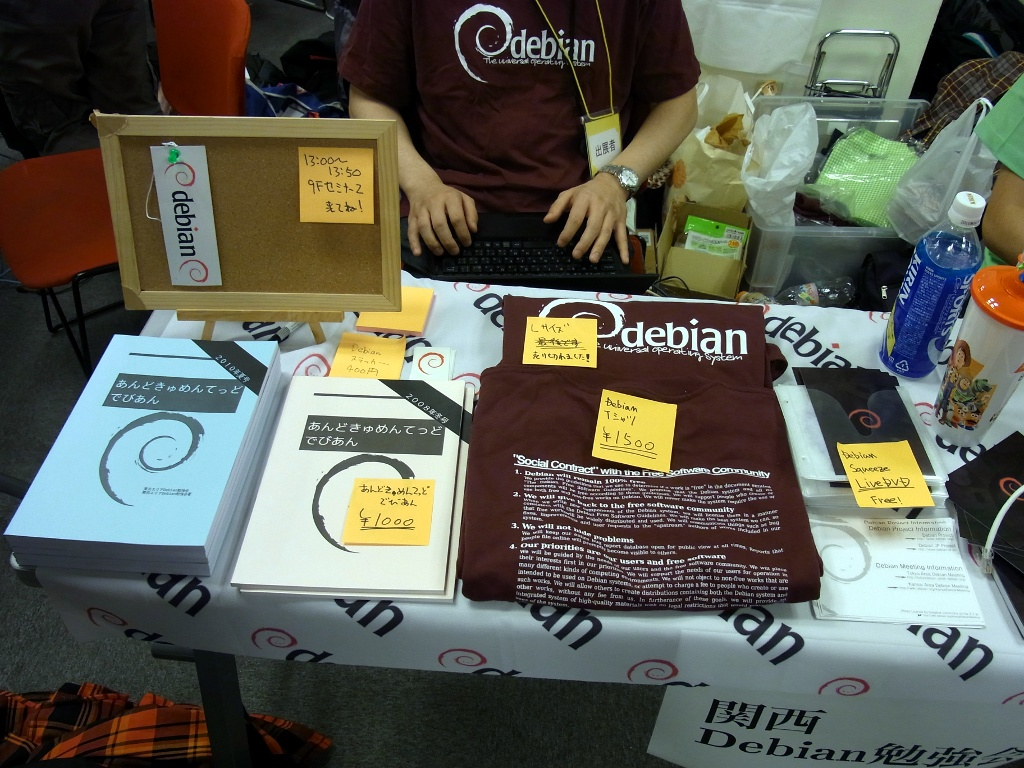
\includegraphics[width=0.30\textwidth]{image201012/kof1.jpg}
    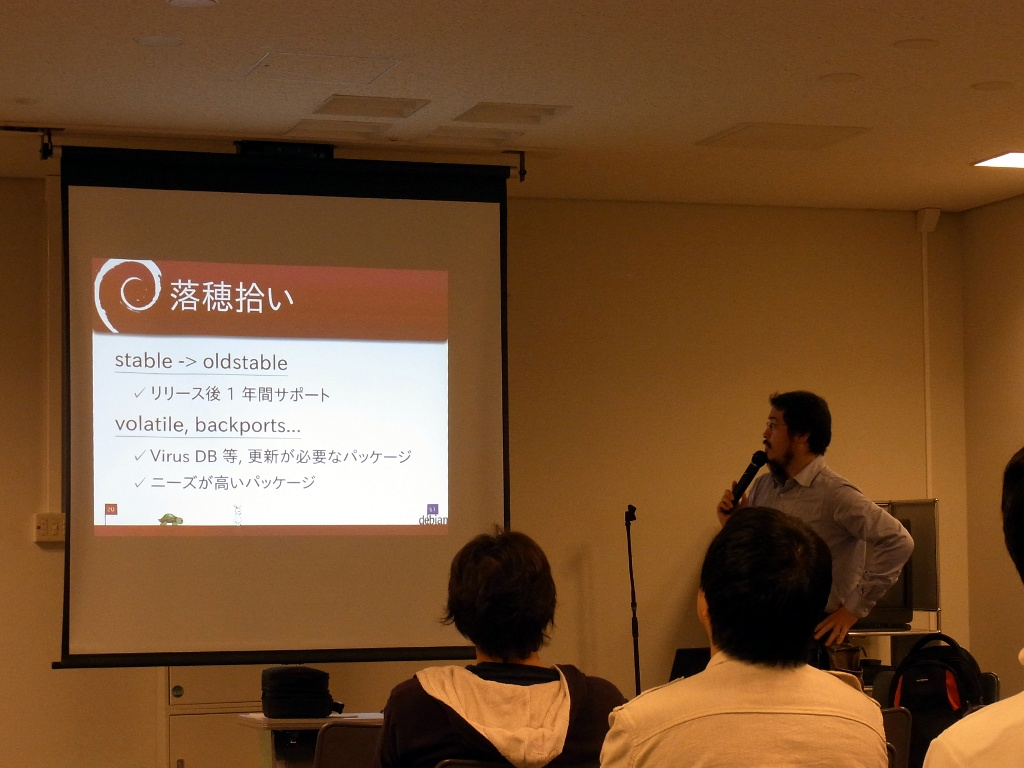
\includegraphics[width=0.30\textwidth]{image201012/kof2.jpg}
    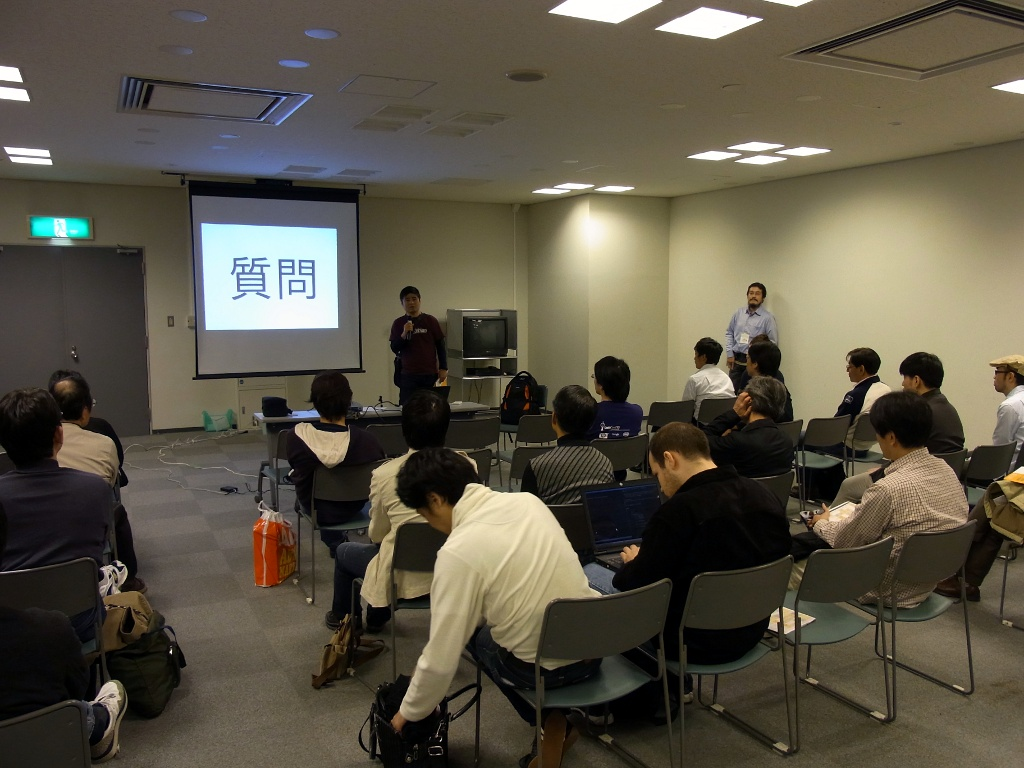
\includegraphics[width=0.30\textwidth]{image201012/kof4.jpg}
    \caption{ブース展示とセッションの様子}
\end{figure}


\subsection{第 70 回東京エリア Debian 勉強会}

11月20日に第70回東京エリアDebian勉強会が開かれました。

11月のテーマはファイルシステムで、実用段階に入ってきたExt4、次世代のファ
イルシステムとして期待されてるNILFS、BtrFS、分散ファイルシステムのCEPHに
ついての発表があり、最近のファイルシステムについて、これだけまとまった資
料はなかなか無いと思うので興味がある方は資料
\footnote{\url{http://tokyodebian.alioth.debian.org/pdf/debianmeetingresume201011.pdf}}
をご覧ください。

個人的にはReiserFSを使っていて、次の乗り換え先としてBtrFSに期待をしている
のですが、資料を読んでNILFSもいいのではと思いました。常用環境としてはまだ
苦しそうなので先の話ですが期待したいところです。

また、日本でのDebConf誘致・開催に先立ち、まずMiniConfから始めようというこ
とで進められているDebian Miniconf in Japanについてのブレストも引き続き行
われたそうです。

\dancersection{事前課題}{Debian JP}

今回は以下の課題を設定しました。
%
\begin{quote}
    \begin{screen}
「2011年の関西 Debian 勉強会で発表する (されてほしい) トピック」を 3 つ挙げてください
    \end{screen}
\end{quote}
%
参加者の皆さんによる回答は以下の通りです。

\begin{prework}{ 川江 }

 \begin{enumerate}
  \item IPv6について
  \item HTML5について
  \item KVMについて
 \end{enumerate}

\end{prework}


\begin{prework}{ 上川純一 }

ひょっとすると参加かも

\end{prework}


\begin{prework}{ 森山京平 }

\begin{itemize}
 \item Vyattaについて。
 \item Debianでねっとわーく。
 \item LinuxプロセスマイグレーションをDebianで行う方法について。
\end{itemize}

\end{prework}


\begin{prework}{ 甲斐正三 }

発表して欲しいトピック

 \begin{itemize}
  \item Squeeze上での日本語TeX環境構築(できればtexworksで)
 \end{itemize}

\end{prework}


\begin{prework}{ のがたじゅん }

パッケージ作成は相変わらず需要が多いような気がします。
ほかはWeb関連と絡めて何か出来ればよいのかなと思ってます。

自分でしゃべるネタとしてはDebian LiveはMultiArchやMultiFS、lxcなどの機能
追加で相変わらず落ち着かないので、新しいことを発表できるかと思います。

\end{prework}


\begin{prework}{ かわだてつたろう }
  \begin{itemize}
  \item ドキュメント
    \begin{itemize}
    \item マニュアル、翻訳、査読などドキュメント全般にまつわること
    \end{itemize}
  \item ライセンス
    \begin{itemize}
    \item DFSG に適合するライセンス、しないライセンス
    \item 適合するライセンスでもそれぞれの違い
    \item 適合しないライセンスの問題点
    \end{itemize}
  \item リリースサイクル
    \begin{itemize}
    \item wheezy から固定リリースサイクルになってどのような変化があったのか
    \end{itemize}
  \end{itemize}
\end{prework}

\begin{prework}{ dictoss(杉本 典充) }

 \begin{itemize}
  \item Debianのカーネル対決。(kLinuxとkFreeBSD)
 \end{itemize}

\end{prework}



\begin{prework}{ 山田 洋平 }

 \begin{itemize}
  \item Debian パッケージの大分類「セクション」、または「GNU R とは何か」
  \item 組み込み開発のための Debian, Emdebian か何か
  \item X11 のウィンドウマネジャですが何か。
 \end{itemize}

\end{prework}

\begin{prework}{ 山下康成 }

 \begin{itemize}
  \item apt V.S. aptitude
  \item nano V.S. vim V.S. emacs etc.etc.
  \item bash V.S. dash
 \end{itemize}
全部、宗教戦争?

\end{prework}

\begin{prework}{ 佐々木洋平 }

 \begin{itemize}
  \item 4--6月は開発者養成虎の穴、のようなルーチンワーク(ライセンスの確認、基本的なパッケージ作成/管理)
  \item OSC/KOF のセッションでは素人(?)向けと開発者(含む予備軍)向け、の二つやりませんか?
  \item 他の勉強会とのクロスセッション. Emacs とか Gentoo とか...
 \end{itemize}
と、リソース考えず言ってみるテスト。

\end{prework}

\begin{prework}{ 木下 }

 \begin{itemize}
  \item 32bitOSから64bitOSへの移行関連
  \item x86系最新プラットフォームのサポート関連
  \item Debian最新バージョン情報関連
 \end{itemize}

\end{prework}

\begin{prework}{ lurdan }

 \begin{itemize}
  \item ゆるい分科会的なしかけを取り入れるのはどうかなぁ
  \item 使いまわせる定番セッションの雛形資料を作って育てていくとか
  \item 今年は一回しかできなかったpuppetネタをもう少しやりたいかも
 \end{itemize}

\end{prework}

\begin{prework}{ 松澤二郎 }

Debian 勉強会の雰囲気をよく把握できていないので的外れな回答になっているかもしれませんが、入門者向けのテーマを扱っていただけるとたいへん嬉しく思います。
例えば、

\begin{itemize}
\item パッケージ作成講座や、
\item 今日からあなたもdebian翻訳者とか、
\item 渦巻きは何なのか
\end{itemize}
など、初心者が知りたいことはたくさんあると思うので、そういうのは入り易くて嬉しいですね。それで、気がついたらDebianプロジェクトに巻き込まれてると。

\end{prework}

\dancersection{Proxmox VE の紹介}{森山京平}
\label{sec:moriyama}
\subsection{自己紹介・経歴・概要}
森山 京平(23)\\
\\
NAIST(奈良の森の中の大学院)\\
Ubuntu User\\
Debianは、サーバ用途でしか触ったことがない。\\
最近は、もっぱら、仮想化技術に興味をもち、KVM を触って自己満足の世界にひ
たっている。某プロジェクト\footnote{AI3 \url{http://www.ai3.net}}のネッ
トワークエンジニア兼サーバエンジニアに任命され、四苦八苦しながらネットワー
ク・サーバの運用と管理を行っている。今年 AI3 Project では、10 年ほど運用
してきたサーバ(物理マシン)のリプレイスを行うようになった。そこで、近年
話題になっている、仮想化技術を用いて、サーバの台数を減らし、可用性を増す
ことを試みた。機器の設置や、dom0(仮想化のベースとなるサーバ)の設定は、
ほぼ終了。仮想マシンで実行するサービスのテストも無事に終わった。今後、次々
に移行していく予定である。KVM を用いて完全仮想化を行うという要求があった
ので、どうしようと迷っていた所、Debian ベースで開発が進んでいる、
ProxmoxVE という OSS に出会い、それを採用させて頂いた。今回は、その
ProxmoxVE について簡単にご説明させていただこうと思う。

\subsection{Proxmoc VEとは}
ProxmoxVEとは、Proxmox Server Solutions GmbH によって開発されている、
Debian ベースでかつ web、cli から仮想マシンを操作できる KVM\&OpenVZ マネー
ジメントツールである。perl と shell を使い qemu や kvm コマンドをうまく
組み合わせて web 上からの操作を可能にしている。競合しているツールとして
同じく web から操作できる KVM のマネージメントツールの karesansui がある。
こちらは国内産であり、100\%PurePython で書かれている。優位性云々は、
karesansui をあまりあたったことがないのでわからない。ProxmoxVE のスター
トは、メールゲートウェイの仮想化を行い、セキュリティを高める目的の仮想化
環境である proxmox という OSS からスタートしている。proxmox から得た知見
を proxmox VEにも適用している。現在の最新バージョンは、1.7 であり、2.0
のリリースが予定されている。ダウンロードは \url{http://www.proxmox.com/}
からできる。

\subsection{インストール}
さて、インストールの方法を説明したい。そのまえに、dom0 マシンに対しての
要求がある。KVM による完全仮想化を実現するために、お持ちのマシンの CPU
が Intel-VT もしくは AMD-V に対応しておかなければならない。もしも、
OpenVZ のみを使うのであれば、それらは、必須ではない。しかしながら、パフォー
マンスとしては、完全仮想化であるほうが、優位であると参考までに覚えておいていただきたい。

\subsubsection{ダウンロード}
ProxmoxVE のイメージをダウンロードする。\url{http://www.proxmox.com/} こ
こから donwnload リンクをたどって行くと iso をダウンロードできる。ダウン
ロードした iso を CD なり DVD に焼く。

\subsubsection{ProxmoVE のインストール}
インストール手順は、至ってシンプル。マシンの性能にもよるが、15 分程度で仮想環境が手に入る。

\subsection{web インターフェースからの各種操作}
ProxmoxVE では、基本的に操作を web インターフェース上から行うように設計
されている。ログイン画面からログインを行うことで、Web 管理コンソールに入ることができる。ログインを終えると、ホストマシンのカレントステータスが表示される。\footnote{CPU、メモリ、カーネルのバージョンなど}

\subsubsection{VM マネージャ}
VM マネージャの欄には、仮想マシン、テンプレート、ISO イメージという項目
が存在する。仮想マシンでは、仮想マシンの状態、作成、マイグレートの操作を
行うことができ、テンプレートでは、OpenVZ のテンプレートに関する操作がで
きる。また、ISO イメージにおいては、OS のインストールディスクのイメージ
をアップロードできる。テンプレートは OpenVZ から、ISOイメージは KVM から用いる。

\paragraph{リスト}
ここから、仮想マシンのそれぞれのメンテナンスタスク、カレントステータスを確認することができる。

\subparagraph{仮想マシンの設定}
実行中の仮想マシンの欄をクリックすることで仮想マシンの設定画面に遷移する。仮想マシンの操作や設定はここから行う。

\begin{itemize}
 \item 仮想マシンの設定[仮想マシンのディスク領域、メモリ、スワップなどの設定]
 \item 仮想マシン削除[仮想マシンの削除をおこなう(復元不可)]
 \item 仮想マシン起動[仮想マシンの起動をおこなう]
 \item 仮想マシン再起動[仮想マシンの強制再起動をおこなう]
 \item 仮想マシンシャットダウン[仮想マシンの強制シャットダウンを行う]
 \item 仮想マシン停止(サスペンド?)[仮想マシンのサスペンドをおこなう(未実装?)]
 \item VNC コンソールへのアクセス[JAVA アプレット-VNC でコンソールへアクセスする]
\end{itemize}

\paragraph{作成}
仮想マシンの作成をおこなう。KVM に対応していれば、KVM の項目が出てくる、
そうでなければ、タイプの欄に OpenVZ の項目しか出てこない。それぞれのパラ
メータの設定おこない、”作成する”をクリックすることで、仮想マシンの作成をおこなえる。

\paragraph{マイグレート}
ProxmoxVEでは、CLI から pveca コマンドを用いることでクラスタリングを行う
ことができる。クラスタリングを行った物理マシン間で仮想マシンのマイグレー
トが可能である。今回は、端折らせていただくが、物理マシンのメンテナンスの
際に役立つ機能である。

仮想マシンの項目から、ほとんどの管理を行うことができる、その点が
ProxmoxVE の素晴らしいとこである。詳細な管理や設定を行いたい場合には、
CLI(ssh によるアクセス)でおこなう。CLI のベースは debian であるので、かなり使いやすい印象をうけた。

\subsubsection{設定}
設定には、システム、ストレージ、バックアップの項目が存在する。

\paragraph{システム}
ネットワーク、DNS、時刻、管理、オプションの項目があり、ネットワークでは、
おもにネットワークインターフェースの設定を行う。DNS では、DNS の設定を行
い、サード DNS サーバまで設定を行える。時刻は、時間帯の設定(JST など)
の設定を行う。NTP サーバの設定ができるかと思ったらそうではなく、もし特定
の NTP サーバの設定を行いたい場合は、CLI からの設定が必要であるように思
う(未確認)。管理の項目からは、管理者の E-mail、パスワードの設定が行え
る。オプションからは、言語とキーボード、HTTP プロキシの設定を行える。

\subparagraph{ストレージ}
ストレージの設定を行う。ストレージの追加削除を行う。iSCSI、NFS、LVMグルー
プ、ディレクトリの参照をおこなうことが可能である。

\subparagraph{バックアップ}
ストレージの項目から、バックアップストレージの指定があれば、ここから、バックアップの設定をおこなうことができる。定期的な仮想マシンのバックアップを行うことができる。

\paragraph{管理}
管理の項目には、サーバ、ログ、クラスタがある。

\subparagraph{サーバ}
サーバのサービスの起動、停止、再起動を行うことができる。SSL証明書もここからダウンロードできる。またサーバそのものの再起動、シャットダウンも行える。

\subparagraph{ログ}
タスクのログ、syslog の確認を行えることは、認識しており、仮想化初心者ユー
ザの敷居を低くする有用な OSS であるかと思う。もし、詳細をしりたい方がい
らっしゃれば、ProxmoxVE の Wiki:\url{http://pve.proxmox.com/wiki/Main_Page}を参照していただけたらと思う。

\dancersection{%
  関西 Debian 勉強会\newline2010年度各種イベント開催実績と総括}{%
  倉敷・佐々木・野方}
%\index{2010ねん@2010年}
%\index{かんさいでびあん@関西Debian勉強会}

\subsection{運営状況}

\subsubsection{勉強会全体}

毎月のセッションについてですが、 %
勉強会の常連さんやイベント等で交流のある方に講師を依頼したりすることで、 %
参加者が関心を持っている様々な分野のネタを勉強会で行なう事ができました。
その反面 Debian との関連性に薄いネタが増えている、という指摘も受けています
\footnote{ネタ自体は Debian に絡められるのに, あんまり関連性について触れられていない, 等}。%
これは我々運営側が講師に依頼する際にもっと明確にお願いすべき事柄の様な気もします。%
今後の反省材料としたい所です。
また、今回の事前課題で複数の方が提出されている通り、%
定番のネタ(Debian 入門的なお話やライセンス、パッケージ作成等)を%
雑誌のように毎年繰り返すことも考えてみたい所です。

講師については、%
継続して参加者して下さる常連さんへの講師依頼をする中で、%
その方が勉強会の運営側へ参加して下さったり、という嬉しい事もありました。
また、Ubuntu コミュニティとの交流があったり、という感じでした。
人の輪がこうして広がっていくのは嬉しいですね。

事前課題については、%
「Debian 勉強会登録システム」の実装と連動してシステム化されたこともあり、%
関西でも毎回の流れにのってきました。%
来年からは東京のように統計をとってもいいかな、と考えています。

イベント参加については、%
今年は春先に OSC Kobe が開催されたため、%
年間通して 3 回分をイベントセッションという形で実施しました。
%
また、勉強会から fork (?) する形でGPG キーサインパーティの実施も定例となりつつあります。
来年も今年通り 3 回の参加を予定しておりますが、%
takaya さんより「ユーザ向け」と「開発者(含むワナビー)向け」の 2 セッションに分けたらどうか、%
との提案もあったりしています。%
当面 4 月の OSC Kobe でのお話になりますが、検討してみたい所です%
\footnote{人的リソースやそもそも二枠取れるのか, 等と気になる課題はありますが}。

{\tt{debian.org}} については、
今年度は佐々木、倉敷の 2 名がめでたく Debian Maintainer になりました。
来年もこの流れを維持できればと思います。

\subsubsection{イベント関連}

例年通り、夏のオープンソースカンファレンスKansai@Kyoto(OSC京都)と、秋の関
西オープンフォーラム(KOF)の出展にくわえ、3月に神戸で開催されたオープンソー
スカンファレンスKansai@Kobe(OSC神戸)にも参加しました。

そしてOSC京都とKOFでは、佐々木さんが中心となりGPGキーサインパーティを開催
しました。

セッションの内容については、OSC神戸やKOFでは最近のDebian関連情報を伝える
軽めのセッション、OSC京都ではパッケージのバックポート講座を開きましたが、
情報系より手を動かすセッションのほうが反響があったので、ハンズオン的なこ
とを増やしていければと思います。

イベントについてはFLOSS関連のイベントが年2回から3回に増えたことと、GPGキー
サインパーティの担当、イベント側のスタッフとして参加など、リソースが若干
厳しくなってきたのでなにかいいバランスを取ることを考えたほうがいいのかも
しれません。


\subsection{開催実績}

関西Debian勉強会の出席状況を確認してみましょう。
グラフで見ると\fgref{fig:kansaipeoplechart}になります。
表で見ると\tbref{tab:count2010kansai} です。

\begin{figure}[h]
 \begin{center}
  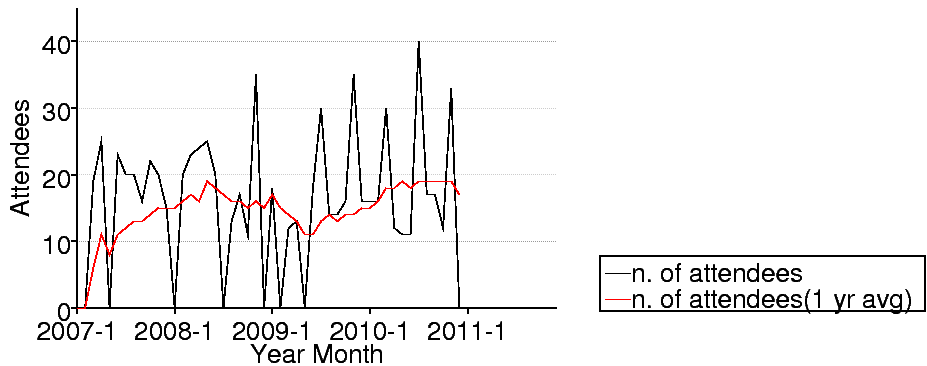
\includegraphics[width=1\hsize]{image201012/memberanalysis/kansai.png}
 \end{center}
\caption{関西の参加人数推移}
\label{fig:kansaipeoplechart}
\end{figure}

\begin{table}
\begin{minipage}{0.5\hsize}
 \caption{関西Debian勉強会参加人数(2007年)}\label{tab:count2007kansai}
 \begin{center}
  \begin{tabular}{|l|c|p{10em}|}
 \hline
 & 参加人数 & 内容 \\
 \hline
2007年3月 & 19 & 開催にあたり \\
2007年4月 & 25 & goodbye、youtube、プロジェクトトラッカー\\
2007年6月 & 23 & 社会契約、テーマ、debian/rules、bugreport\\
2007年7月 & 20前後 & OSC-Kansai \\
2007年8月 & 20 & Inkscape、patch、dpatch\\
2007年9月 & 16 & ライブラリ、翻訳、debtorrent\\
2007年10月 & 22& 日本語入力、SPAMフィルタ\\
2007年11月 & 20前後 & KOF \\
2007年12月 & 15& 忘年会、iPod touch\\
 \hline
  \end{tabular}
 \end{center}
\end{minipage}
\begin{minipage}{0.5\hsize}
 \caption{関西Debian勉強会参加人数(2008年)}\label{tab:count2008kansai}
 \begin{center}
  \begin{tabular}{|l|c|p{10em}|}
 \hline
 & 参加人数 & 内容 \\
 \hline
2008年2月 & 20 & PC Cluster, GIS, \TeX \\
2008年3月 & 23 & bug report, developer corner, GPG \\
2008年4月 & 24 & coLinux, Debian GNU/kFreeBSD, sid \\
2008年5月 & 25  & ipv6, emacs, ustream.tv\\
2008年6月 & 20  & pbuilder, hotplug, ssl\\
2008年8月 & 13  & coLinux \\
2008年9月 & 17  & debian mentors, ubiquity, DFSG\\
2008年10月 & 11  & cdbs,cdn.debian.or.jp \\
2008年11月 & 35  & KOF \\
2008年12月 & ?  & TeX資料作成ハンズオン\\
 \hline
  \end{tabular}
 \end{center}
\end{minipage}
\begin{minipage}{0.5\hsize}
 \caption{関西Debian勉強会参加人数(2009年)}\label{tab:count2009kansai}
 \begin{center}
  \begin{tabular}{|l|c|p{10em}|}
 \hline
 & 参加人数 & 内容 \\
 \hline
2009年1月 & 18 & DMCK, LT \\
2009年3月 & 12 & Git \\
2009年4月 & 13 & Installing sid, Mancoosi, keysign \\
2009年6月 & 18 & Debian Live, bash\\
2009年7月 & 30? & OSC2009Kansai \\
2009年8月 & 14 & DDTSS, lintian \\
2009年9月 & 14 & reportbug, debian mentors\\
2009年10月 & 16 & gdb, packaging \\
2009年11月 & 35 & KOF2009 \\
2009年12月 & 16 & GPS program, OpenStreetMap \\
 \hline
  \end{tabular}
 \end{center}
\end{minipage}
\begin{minipage}{0.5\hsize}
 \caption{関西Debian勉強会参加人数(2010年)}\label{tab:count2010kansai}
 \begin{center}
  \begin{tabular}{|l|c|p{10em}|}
 \hline
 & 参加人数 & 内容 \\
 \hline
2010年1月 & 16 & Xen, 2010年企画 \\
2010年2月 & 16 & レンタルサーバでの利用, GAE \\
2010年3月 & 30? & OSC2010Kobe \\
2010年4月 & 12 & デスクトップ環境, 正規表現 \\
2010年5月 & 11 & ubuntu, squeeze \\
2010年6月 & 11 & debhelper7, cdbs, puppet \\
2010年7月 & 40? & OSC2010Kyoto \\
2010年8月 & 17 & emdebian, kFreeBSD \\
2010年9月 & 17 & タイルWM \\
2010年10月 & 12 & initramfs, debian live \\
2010年11月 & 33 & KOF2010 \\
2010年12月 & 14 & Proxmox, annual review \\
 \hline
  \end{tabular}
 \end{center}
\end{minipage}
\end{table}

\clearpage

\dancersection{今後の予定}{Debian JP}

\subsection{次回の関西Debian勉強会}
次回の関西 Debian 勉強会は1月23日(日)、大阪港区区民センター楓の間にて行う
予定です。いつもの福島区民センターではないのでお気をつけください。

発表については未定ですので、みなさまの発表をお待ちしております。


% 冊子にするために、4の倍数にする必要がある。
% そのための調整
%\dancersection{メモ}{}
%\mbox{}\newpage

%\printindex
 \cleartooddpage

 \begin{minipage}[b]{0.2\hsize}
  \rotatebox{90}{\fontsize{80}{80} {\gt 関西 Debian 勉強会} }
 \end{minipage}
 \begin{minipage}[b]{0.8\hsize}

 \vspace*{15cm}
 \rule{\hsize}{1mm}
 \vspace{2mm}
 
\includegraphics[width=2cm]{image200502/openlogo-nd.eps}
 \noindent \Large \bf Debian 勉強会資料\\ \\
 \noindent \normalfont \debmtgyear{}年\debmtgmonth{}月\debmtgdate{}日 \hspace{5mm}  初版第1刷発行\\
 \noindent \normalfont 関西 Debian 勉強会 (編集・印刷・発行)\\
 \rule{\hsize}{1mm}
 \end{minipage}

\end{document}
